\chapter{ Specificari Back-end}
\label{chap:ch5}

\par Pe partea de back end sunt prezente doua servere, unul scris in JavaScript cu ajutorul framework-ului Node js care serveste partea de front-end cu toate datele de care are nevoie si un server scris in Python cu ajutorul framework-ului Flask cu ajutorul caruia aflu filme recomandate pentru un film sau o lista  de filme.

\section{Baza de date}
\label{sec:ch5sec1}

\begin{figure}[htbp]
\centerline{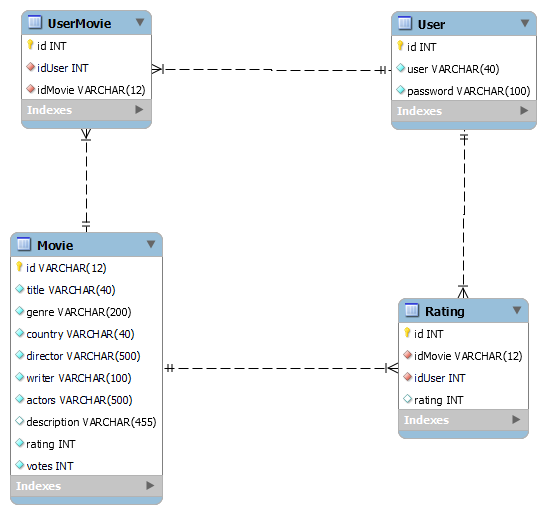
\includegraphics[width=10cm, height=10cm]{figures/diagrama db.png}}
\caption{Diagrama baza de date.}
\label{fig}
\end{figure}

\par Un lucru foarte important in dezvoltarea aplicatiei a fost alegerea bazei de date, am optat pentru pentru MySql versiunea 8.0. In tabelul de User voi salva datele de inregisrare a unui utilizator , in tabelul  Movie sunt prezente datele care descriu un film prin colloanele:title,genre,country,directors,writers,actors,description,votes si rating, in tabelul Rating salvez datele unui rating dat de un user pe laga valoare ratingului salvez si id-urile de la film si user pentru a stii cine da rating si la ce film totodata pe partea de back-end fac si o actualizare a rating ului si numarului de voturi din tabelul Movie asta pentru o a face aplicatia sa se miste mai rapid, iar in tabelul UserMovie salvez id ul de la un user si id ul de la un film reprezentand un film pe care utilizatorul l-a vizualizat.

\section{Server Node Js}
\label{sec:ch5sec1}

\par Serverul de Node Js il folosesc pentru a face inregistrare, login, returanrea tuturor filmelor care contin un numit sub titlu, adaugarea unui film la lista utilizatorului, returnarea a tuturor filmelor unui utilizator si adaugarea de rating a unui film. Cu ajutorul pachetului Express stabilesc rutele si pornesc serverul. Cand se face un request pe o ruta, se apeleaza functia asignata din Service, care are rol de a modela datele in functie de cum avem nevoie. Pentru a comunica cu baza de date ne folosim de Repository, acesta face legatura cu baza de date.

\subsection{Inregistrare}
\par Procesul de inregistrare este unul simplu, pasii fiind urmatorii:
\begin{enumerate}
  \item The individual entries are indicated with a black dot, a so-called bullet.
  \item The text in the entries may be of any length.
\end{enumerate}